\documentclass[a4paper,12pt]{article} 

%%%%%%%%%%%%%%%%%%%%%%%%%%%%%%%%%%%%%%%%%%%%%%%%%%%%%%%%%%%%%%%%%%%%%%%%%%%%
\usepackage[utf8]{inputenc}
\usepackage[spanish]{babel}
\usepackage{amsmath}
\usepackage{amsfonts}
\usepackage{amssymb} 
\usepackage{graphicx} 
\usepackage{hyperref} 
\usepackage{wrapfig}
\usepackage{enumitem}
\usepackage{blindtext}
\usepackage{fancyhdr}
\usepackage{float}
\usepackage{eurosym}
\usepackage{color}
\usepackage{titling}
\usepackage{amssymb, amsmath, amsbsy} % simbolitos
 \usepackage{upgreek} % para poner letras griegas sin cursiva
 \usepackage{cancel} % para tachar
 \usepackage{mathdots} % para el comando \iddots
 \usepackage{mathrsfs} % para formato de letra
\usepackage{stackrel} % para el comando \stackbin
\usepackage{lipsum}
\usepackage{tocbibind}
\usepackage[T1]{fontenc}
\usepackage[left=3cm,right=3cm,top=3cm,bottom=4cm]{geometry}
\pagestyle{fancy}
%%%%%%%%%%%%%%%%%%%%%% CABECERAS %%%%%%%%%%%%%%%%%%%%%%%%%%%%%%%%%%%%%%%%%%%
\newcommand{\hsp}{\hspace{20pt}}
\newcommand{\HRule}{\rule{\linewidth}{0.5mm}}
\headheight=50pt
\newcommand{\vacio}{\textcolor{white}{holacaracola}}
%%% NUMERACION DE ECUACIONES
\renewcommand{\theequation}{\thesection.\arabic{equation}}
% COLOR AZUL PARA TEXTOS EN PORTADA
\definecolor{azulportada}{rgb}{0.16, 0.32, 0.75}
% Azul para textos de headings
\definecolor{azulinterior}{rgb}{0.0, 0.2, 0.6}

%%%%%%%%%%%%%%%%%%% DATOS DEL PROYECTO %%%%%%%%%%%%%%%%%%%%%%%%%%%%%%%%%%%%%
\title{Actividad 9}
\author{}
\newcommand{\director}{Carlos Lizárraga Celaya}

\begin{document}
\begin{titlepage}
\begin{center}
\vspace{1cm}

\includegraphics[width=5.5cm]{unison-logo.png}
\\[0.5cm]
{\fontfamily{phv}\fontsize{24}{6}\selectfont{UNIVERSIDAD DE SONORA}}\\
[1em]
{\fontfamily{phv}\fontsize{16}{5}\selectfont{DEPARTAMENTO DE FÍSICA}}\\
[4em]
\textcolor{azulportada}
{\fontfamily{phv}\fontsize{30}{5}\selectfont{\textsc{\thetitle}}}\\
% Autor del trabajo de investigación
[1cm]
{\fontfamily{phv}\fontsize{16}{5}\selectfont{Alumno:}}\\
[0.2cm]
%Equipo sfdsfshkfhsfhsjfs
{\fontfamily{phv}\fontsize{14}{5}\selectfont{Luis Alfonso Torres Flores}}\\
[1cm]
%{\Huge\textbf{\thetitle}}\\
{\fontfamily{phv}\fontsize{16}{5}\selectfont{Profesor}}\\
[0.2cm]
{\fontfamily{phv}\fontsize{16}{5}\selectfont{\director}}\\
[4.5cm]
{\fontfamily{phv}\fontsize{14}{5}\selectfont{19 de Mayo de 2017}}\\
[4cm]
\end{center}
\restoregeometry
\end{titlepage}

\newpage
%%%Encabezamiento y pie de página
\renewcommand{\headrulewidth}{0.5pt}
\fancyhead[R]{
	\textcolor{azulinterior}{\fontfamily{phv}\fontsize{14}{4}\selectfont{\textbf{\thetitle}}}\\
\textcolor{azulportada}{\fontfamily{phv}\fontsize{10}{3}\selectfont{Curso de Fisica computacional}}\\
{\fontfamily{phv}\fontsize{10}{3}\selectfont{\theauthor}}}
\fancyhead[L]{\vacio}
\newpage
%-------------------------------------------------------
\section*{Breve resumen}
\noindent
Al igual que en la actividad anterior que generamos un gif, también podemos crear archivos e videos mp4, como lo será en esta actividad.

\section*{Introducción}
\noindent
En este reporte mostraremos el código empleado. Dicho código tiene como función mostrar distintos pasos para la obtención de la animación que deseamos generar como un archivo mp4. El archivo, al igual que la actividad anterior, muestra el efecto mariposa. En el código iremos generando diversas imágenes que mostraremos más adelante en el orden en el que aparecerán al abrir y usar el archivo de Python correspondiente a este trabajo.

Para poder realizar el archivo mp4 se necesita la instalación de pynamical, cosa que necesitaremos si podemos observar los archivos que importamos al inicio de nuestro código. También se pudo encontrar algunos problemas a la hora de generar el archivo deseado debido a la falta de un código, mismo que se encuentra ahora en el trabajo. Si revisamos el código cuidadosamente podremos observar que podemos cambiar algunas características a placer, tal y como es el color de las gráficas y del video mismo, por lo que en cierto grado puede ser modificado a gusto.

\section*{Codigo}
import pynamical
from pynamical import simulate, save\_fig, phase\_diagram, phase\_diagram\_3d
import pandas as pd, numpy as np, matplotlib.pyplot as plt, IPython.display as IPdisplay
\%matplotlib inline

title\_font = pynamical.get\_title\_font()
label\_font = pynamical.get\_label\_font()

\# draw a phase diagram for 100 generations for the growth rate parameter 2.9
\# it shows points converging on 0.655 because the logistic map has a fixed-point attractor at 0.655 when r=2.9
pops = simulate(num\_gens=100, rate\_min=2.9, num\_rates=1, num\_discard=100)
phase\_diagram(pops, title='Logistic Map Attractor, r=2.9', size=20)

\# draw a phase diagram for 100 generations for the growth rate parameter 3.5
\# it shows 4 points because the logistic map has a period of 4 when r=3.5
pops = simulate(num\_gens=100, rate\_min=3.5, num\_rates=1, num\_discard=100)
phase\_diagram(pops, title='Logistic Map Attractor, r=3.5', size=20)

\# draw a phase diagram for 100 generations for the growth rate parameter 3.56
\# it shows 8 points because the logistic map has a period of 8 when r=3.56
pops = simulate(num\_gens=100, rate\_min=3.56, num\_rates=1, num\_discard=100)
phase\_diagram(pops, title='Logistic Map Attractor, r=3.56', size=20)

\# draw a phase diagram for 100 generations for the growth rate parameter 3.57
\# it shows n points because the logistic map has a period of n when r=3.57
pops = simulate(num\_gens=100, rate\_min=3.57, num\_rates=1, num\_discard=100)
phase\_diagram(pops, title='Logistic Map Attractor, r=3.57', size=20)

\# draw a phase diagram for 2,000 generations for the growth rate parameter 3.9
\# the plot reveals the strange attractor - the logistic map is chaotic when r=3.9
pops = simulate(num\_gens=2000, rate\_min=3.9, num\_rates=1)
phase\_diagram(pops, xmin=0.25, xmax=0.75, ymin=0.8, ymax=1.01, size=20, title='Logistic Map Attractor, r=3.9')

\# draw a phase diagram for 2,000 generations across 50 growth rate steps from 3.6 to 4.0
\# each chaotic growth rate has its own parabola
pops = simulate(num\_gens=2000, rate\_min=3.6, rate\_max=4.0, num\_rates=50)
phase\_diagram(pops, xmin=0.25, xmax=0.75, ymin=0.8, ymax=1.01, size=7, 
              title='Logistic Map Attractor, r=3.6 to r=4.0', color='viridis')
              
\# sometimes it is hard to tell if a time series is chaotic or random
\# generate two time series of 1,000 steps, one chaotic and one random
\# generate 30,000 time steps for the chaotic series but only keep the final 1,000 (when system is fully evolved)
total\_gens = 30000
gens = 1000
np.random.seed(1)

chaos\_pops = simulate(num\_gens=total\_gens, rate\_min=3.99, num\_rates=1)
chaos\_pops = chaos\_pops.iloc[total\_gens-gens:].reset\_index().drop(labels='index', axis=1)

random\_pops = pd.DataFrame(np.random.random(gens), columns=['value'])
time\_series = pd.concat([chaos\_pops, random\_pops], axis=1)
time\_series.columns = ['chaos', 'random']
time\_series.head()

\# plot the chaotic and random time series to show how they are sometimes tough to differentiate
ax = time\_series.plot(kind='line', figsize=[10, 6], linewidth=3, alpha=0.6, style=['\#003399','\#cc0000'])
ax.grid(True)
ax.set\_xlim(40, 90)
ax.set\_ylim(0, 1)
ax.set\_title('Time Series, Deterministic Chaos vs Random Data', fontproperties=title\_font)
ax.set\_xlabel('Generation', fontproperties=label\_font)
ax.set\_ylabel('Population', fontproperties=label\_font)
ax.legend(loc=3)

save\_fig('chaos-vs-random-line')
plt.show()

\# plot same data as 2D phase diagram instead
pops = pd.concat([chaos\_pops, random\_pops], axis=1)
pops.columns = ['chaos', 'random']
phase\_diagram(pops, size=20, color=['\#003399','\#cc0000'], ymax=1.005, legend=True, 
              filename='logistic-attractor-chaos-random')
              
\# plot same data as 3D phase diagram instead
phase\_diagram\_3d(pops, color=['\#003399','\#cc0000'], filename='logistic-attractor-chaos-random-3d',
                 legend=True, legend\_bbox\_to\_anchor=(0.94, 0.9))
                 
\# plot same data as 3D phase diagram instead
phase\_diagram\_3d(pops, color=['\#003399','\#cc0000'], filename='logistic-attractor-chaos-random-3d',
                 legend=True, legend\_bbox\_to\_anchor=(0.94, 0.9))

\# run logistic model for 4,000 generations across 50 growth rate steps from 3.6 to 4.0
pops = simulate(num\_gens=4000, rate\_min=3.6, rate\_max=4.0, num\_rates=50)

\# phase diagram: each chaotic growth rate has its own strange attractor curling through state space
phase\_diagram\_3d(pops, title='Mapa logistico de atractor de r=3.6 a r=4.0', alpha=0.1, color='inferno', color\_reverse=False, 
                 azim=230, filename='3d-logistic-map-attractor-1',
                 xlabel='Población (t)', ylabel='Población (t+1)', zlabel='Población (t+2)')
                 
\# phase diagram: each chaotic growth rate has its own strange attractor curling through state space
phase\_diagram\_3d(pops, title='Mapa logistico de atractor de r=3.6 a r=4.0', alpha=0.1, color='inferno', color\_reverse=False, 
                 elev=7, azim=320, filename='3d-logistic-map-attractor-2', 
                 xlabel='Población (t)', ylabel='Población (t+1)', zlabel='Población (t+2)')
                 
\# here's an example of the animated phase diagrams that I create in pynamical-demo-3d-animation.ipynb
IPdisplay.Image(url='images/phase-animate/05-logistic-3d-phase-diagram-chaotic-regime.gif')

\section*{Imagenes obtenidas}
\begin{center}
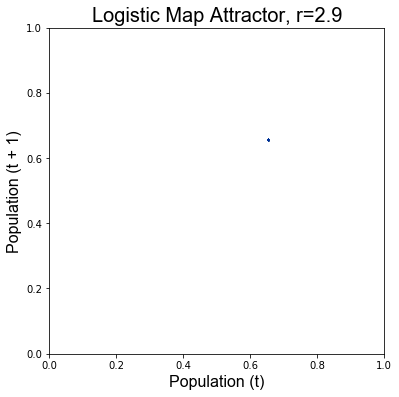
\includegraphics[scale=0.5]{5.png}
\end{center}
\begin{center}
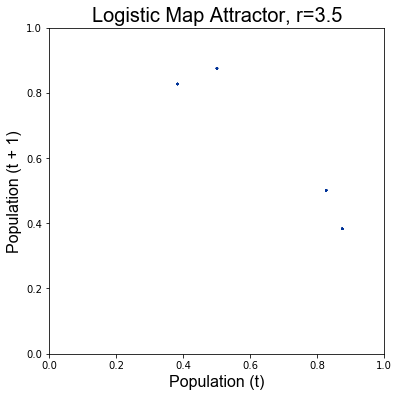
\includegraphics[scale=0.5]{6.png}
\end{center}
\begin{center}
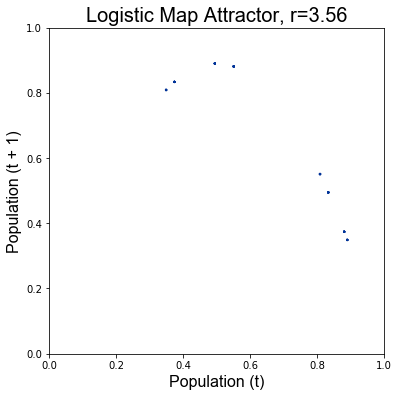
\includegraphics[scale=0.5]{7.png}
\end{center}
\begin{center}
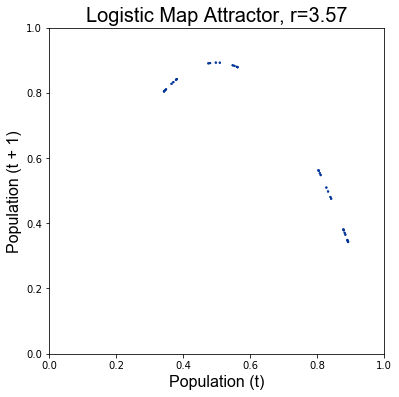
\includegraphics[scale=0.5]{8.png}
\end{center}
\begin{center}
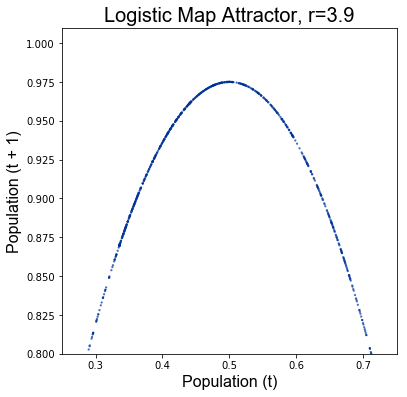
\includegraphics[scale=0.5]{9.png}
\end{center}
\begin{center}
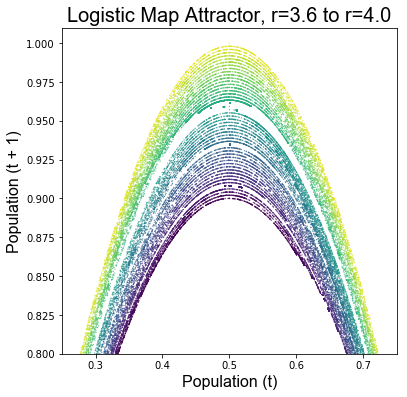
\includegraphics[scale=0.5]{10.png}
\end{center}
\begin{center}
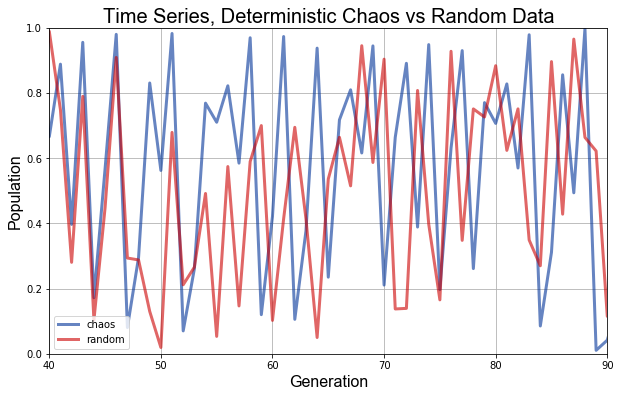
\includegraphics[scale=0.5]{11.png}
\end{center}
\begin{center}
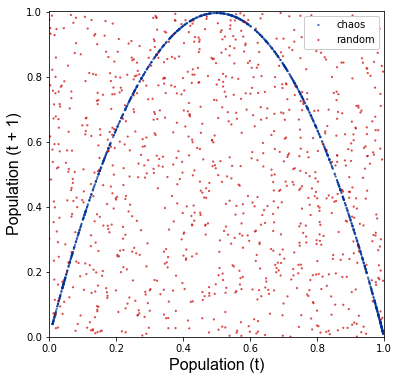
\includegraphics[scale=0.5]{12.png}
\end{center}
\begin{center}
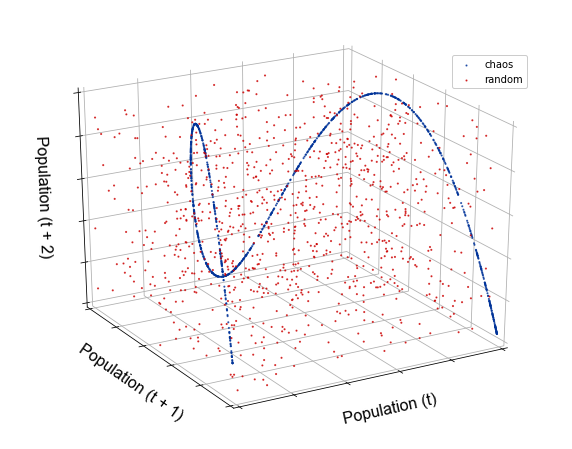
\includegraphics[scale=0.5]{13.png}
\end{center}
\begin{center}
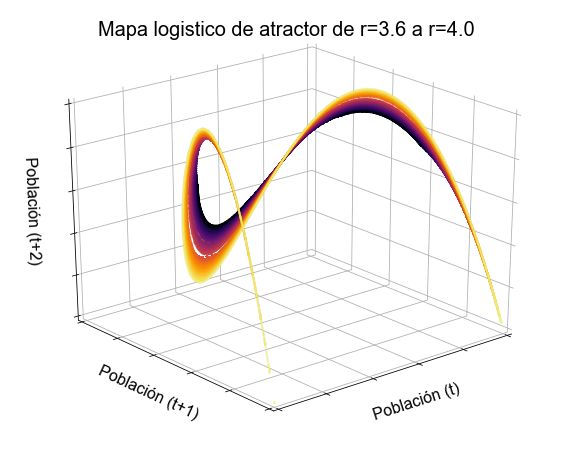
\includegraphics[scale=0.5]{14.png}
\end{center}
\begin{center}
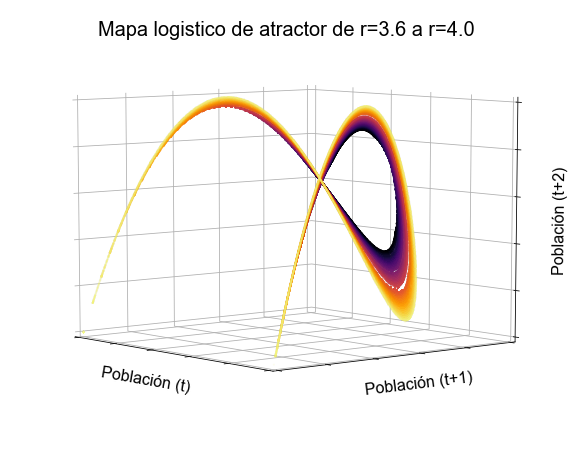
\includegraphics[scale=0.5]{15.png}
\end{center}
\end{document}
